\documentclass{article}
\usepackage{tmlr}

\usepackage{amsmath}
\usepackage{amssymb}
\usepackage{amsthm}
\usepackage{booktabs}
\usepackage{graphicx}
\usepackage{microtype}
\usepackage{url}  % the bibliography emits \url{...}; tmlr.sty does not provide it

\theoremstyle{plain}
\newtheorem{proposition}{Proposition}
\newtheorem{lemma}{Lemma}
\theoremstyle{definition}
\newtheorem{assumption}{Assumption}
\newtheorem{definition}{Definition}

% Generated by scripts/fb_macros_aistats.py -- do not edit by hand.
% Every value is read from a committed result file; see CLAIM_LEDGER_AISTATS.md.
\newcommand{\NumModels}{27}
\newcommand{\NumItems}{1{,}324}
\newcommand{\NumOrderings}{351}
\newcommand{\NumVerifiers}{3}
\newcommand{\NumCells}{8}
\newcommand{\NumRows}{35{,}748}
\newcommand{\MissingRows}{0}
\newcommand{\CommonItems}{1{,}324}
\newcommand{\EmReexecDisagree}{0}
\newcommand{\EmReexecItems}{35{,}748}
\newcommand{\EmAggregateMatch}{175}
\newcommand{\MvAggregateMatch}{168}
\newcommand{\NumSubjectsRescored}{175}
\newcommand{\CellAgreeAll}{1{,}904}
\newcommand{\CellRejectAll}{32{,}685}
\newcommand{\RowsAnyDisagree}{1{,}159}
\newcommand{\DisagreeSbEmSeventeen}{704}
\newcommand{\DisagreeSbEmSeventeenString}{817}
\newcommand{\AuditCorrectAgreeAll}{142}
\newcommand{\AuditNAgreeAll}{144}
\newcommand{\AuditCorrectRejectAll}{0}
\newcommand{\AuditNRejectAll}{223}
\newcommand{\CertEpsZero}{153}
\newcommand{\CertEpsZeroSim}{120}
\newcommand{\CertEpsZeroAudit}{208}
\newcommand{\CertPrereg}{131}
\newcommand{\CertPreregSim}{109}
\newcommand{\CertNoPooling}{0}
\newcommand{\CeilingEm}{280}
\newcommand{\CeilingMv}{263}
\newcommand{\CertKTwoEpsZero}{163}
\newcommand{\CertKTwoPrereg}{143}
\newcommand{\EpsPrereg}{0.01}
\newcommand{\EpsRefDerived}{10.06}
\newcommand{\BreakdownMedian}{0.05769}
\newcommand{\AnchorStringCombined}{84}
\newcommand{\AnchorSympyCombined}{89}
\newcommand{\AnchorStringAudit}{101}
\newcommand{\AnchorSympyAudit}{104}
\newcommand{\SimReplicates}{2{,}000}
\newcommand{\SimWorstFwerUnderH}{0}
\newcommand{\SimFwerMisspecified}{0.0675}
\newcommand{\SimFwerPropensityKTwo}{0.185}
\newcommand{\SimScenarios}{9}
\newcommand{\SimMcSeAudit}{0.003491}
\newcommand{\AlphaAudit}{0.025}
\newcommand{\AlphaSample}{0.025}
\newcommand{\SidakTwoLevel}{0.9874}
\newcommand{\CertHoeffding}{100}
\newcommand{\CertSamplingLegacy}{160}
\newcommand{\TestsTotal}{880}
\newcommand{\TestsFunctions}{71}
\newcommand{\TestsCertification}{613}
\newcommand{\TestsManuscriptClaims}{203}
\newcommand{\TestsAnchor}{7}
\newcommand{\AuditBudget}{458}
\newcommand{\ScreenedModels}{2}
\newcommand{\ScreenNRejectAll}{39}
\newcommand{\ScreenNAgreeAll}{100}
\newcommand{\ScreenRho}{0.2}
\newcommand{\ScreenPowerPct}{80}
\newcommand{\ScreenPowerRejectAll}{0.82}
\newcommand{\ScreenPowerAgreeAll}{0.8077}
\newcommand{\LabelsFalsification}{278}
\newcommand{\LabelsCertification}{180}
\newcommand{\ProjectedCertPrereg}{138}
\newcommand{\LmEvalGenerative}{4{,}524}
\newcommand{\LmEvalCoerce}{2{,}936}
\newcommand{\LmEvalCoercePct}{64.9}
\newcommand{\OpenCompassGenerative}{1{,}070}
\newcommand{\OpenCompassCoerce}{158}
\newcommand{\OpenCompassCoercePct}{14.8}
\newcommand{\LightevalGenerative}{37}
\newcommand{\LightevalCoerce}{13}
\newcommand{\SimpleEvalsStringMatch}{6}
\newcommand{\SimpleEvalsCoerce}{4}
\newcommand{\CensusValidTestable}{93}
\newcommand{\CensusValidConfirmed}{93}
\newcommand{\CensusControlN}{100}
\newcommand{\CensusControlClean}{100}


\title{Which Leaderboard Orderings Survive a Human Reader?}
\author{Anonymous}

\begin{document}

\maketitle
% Draft abstract for the TMLR resubmission. All numbers are macros.

\begin{abstract}
A benchmark score is produced by a model and by a verifier that decides what answer the
model's text contains. Only the model is named in the leaderboard. We ask what happens to a
published ranking when a human reader, rather than a string matcher, decides what each
response says.

On the Open LLM Leaderboard's MATH-Hard board, we read all \NumRows{} published responses
from \NumModels{} models with three verifiers: the leaderboard's original 2024 scorer, the
verifier behind its February 2025 re-scoring, and a boxed-answer extractor following the
benchmark's own reference convention. Re-executing the scoring function recorded in the
leaderboard's result files reproduces its published per-item verdicts on \EmReexecItems{} of
\EmReexecItems{} responses, which establishes the identity of the published verifier from
records rather than from agreement. The three verifiers disagree on \RowsAnyDisagree{}
responses, and those responses are where the ranking is decided.

Certifying a ranking from a few hundred human labels requires pooling across models, and
pooling requires an assumption about how far the models may differ where the verifiers agree.
We state that assumption as a single parameter $\varepsilon$, derive an identified range for
each pairwise difference under it, and report certified orderings as a function of
$\varepsilon$ instead of at one chosen value. Of \NumOrderings{} pairwise orderings,
\CertEpsZero{} are certified under exact homogeneity, \CertPrereg{} at the tolerance we
registered before seeing results, and \CertNoPooling{} with no pooling at all. The audit
bounds are design-valid without assuming equal rates across models, and simulation at the
full \NumModels{}-model scale confirms the stated coverage where the assumption holds and
shows it failing where it does not.

Two provenance findings shape what can be claimed. The leaderboard changed its own MATH
verifier in February 2025, so the per-item verdicts it publishes and the scores it displays
come from different scorers. And our own boxed verifier was silently degraded by a
platform-specific defect that reduced symbolic equivalence to string comparison; correcting
it moves the count of disagreeing responses on our earlier subset from
\DisagreeSbEmSeventeenString{} to \DisagreeSbEmSeventeen{}. We report the corrected analysis
together with the defect that produced the earlier numbers.

We release the human labels, the per-cell census of all \NumRows{} responses, the three
verifier configurations with their shared components stated explicitly, and the code that
regenerates every number in this paper.
\end{abstract}


% Draft for the TMLR resubmission. Numbers enter only through macros
% (manuscript/aistats2027/macros.tex, generated by scripts/fb_macros_aistats.py).
% Writing rules applied: no contractions; specifics delivered as ordinary sentences rather
% than colon-led parallel series; no sentence shortened for cadence; no narration of the
% argument's own significance.

\section{Introduction}
\label{sec:intro}

A model was asked how many more euros than pounds Kathy has. It converted both amounts,
compared them, and wrote: ``Kathy has $\boxed{22}$ more euros than pounds. Final Answer: The
final answer is 22. Great job!'' The reference answer is 22. A person reading the response
would mark it correct. The leaderboard recorded it as wrong.

Nothing went wrong with the model. The scorer that produced that verdict looks for one
sentence pattern, ``Final Answer: The final answer is X. I hope it is correct.'', and this
response ended with ``Great job!'' instead. The extraction returned its sentinel for no
answer found, and a response with no answer found is recorded exactly as a response with a
wrong answer. The published score for that model is one item lower, and nothing in the
published output says why.

This is not a rare accident, and it is not confined to one scorer. Every benchmark score is
produced by two components. A model writes text, and a \emph{verifier} decides what answer
that text contains and whether it matches the reference. Only the first component is named in
the leaderboard. The second is a configuration choice that varies between frameworks, between
tasks inside one framework, and over time within a single task: the Open LLM Leaderboard
re-scored its own MATH results in February 2025 with a different verifier, and the published
numbers changed while the model outputs stayed exactly as they were.

The consequence we care about is not that scores are slightly too low. Everyone who has
looked at this already knows that a benchmark score is a lower bound on what a careful reader
would credit, and a uniform downward bias would be a nuisance rather than a problem. The
consequence is that the \emph{ranking} can move. Lower bounds do not order models. If one
model happens to phrase its answers the way the verifier expects and another does not, the
gap between them is partly a fact about formatting conventions and partly a fact about
mathematics, and the published number does not separate them.

\paragraph{What this paper does.}
We take the \NumModels{} models of the Open LLM Leaderboard's MATH-Hard board, with all
\NumItems{} Level-5 items and the leaderboard's own published generations, and ask which of
the \NumOrderings{} pairwise orderings survive when a human reader, rather than a string
matcher, decides what each response says.

Three verifiers read the same responses. The first is the leaderboard's original 2024 scorer,
whose per-item verdicts are published in its own result files. The second is the verifier
behind the leaderboard's current published scores, introduced in the February 2025 re-scoring.
The third extracts the last boxed expression, which is the convention the benchmark's own
reference solutions use. Each response therefore falls into one of eight \emph{cells},
according to which verifiers credited it. The cells where all three agree cover most of the
board. The cells where they disagree, \RowsAnyDisagree{} of \NumRows{} responses, are where
the ranking is decided.

Human labels are expensive, so they go where the disagreement is. We reuse an existing
400-item audit and add a preregistered \AuditBudget{}-label audit stratified by model and
cell. The estimate that the audit supports is not a correction to each model's score. It is a
bound on each pairwise difference, and whether that bound excludes zero.

\paragraph{The assumption, stated in advance.}
A small audit cannot measure every model separately in every cell. Certifying a ranking from
a few hundred labels requires pooling, and pooling requires an assumption: that in the cells
where the verifiers agree, the rate at which a human reader overrules them does not vary too
much across models. We write this as $H(\varepsilon)$, where $\varepsilon$ bounds the spread
across models, and we report results as a function of $\varepsilon$ rather than at a single
convenient value.

At $\varepsilon = 0$, which is exact homogeneity, the existing audit certifies \CertEpsZero{}
of \NumOrderings{} orderings. At the tolerance we registered before seeing any result,
$\varepsilon = \EpsPrereg$, it certifies \CertPrereg{}. Without pooling at all, it certifies
\CertNoPooling{}. The assumption carries the result, and saying so plainly is part of the
contribution rather than a caveat attached to it.

We also report what $\varepsilon = 0$ actually means. Because $\varepsilon$ constrains
realized fractions over finitely many responses, exact homogeneity is unattainable whenever
the underlying rate is strictly between zero and one; sampling variation alone spreads the
per-model fractions. In simulation at the full scale of this board, an analysis conducted at
$\varepsilon = 0$ against a world with homogeneous underlying rates exceeded its nominal error
rate, and a tolerance of \EpsPrereg{} restored it. We therefore treat $\varepsilon = 0$ as an
idealization that belongs at one end of a curve, and never as a headline.

\paragraph{What we found along the way.}
Two findings emerged from checking the provenance of the verdicts rather than from the
analysis itself, and both change what can be claimed.

First, the leaderboard's published per-item verdicts are reproducible. Re-executing the
scoring function recorded in the leaderboard's own result files reproduces the published
verdict on \EmReexecItems{} of \EmReexecItems{} responses. The identity of the published
verifier is therefore established from the leaderboard's records rather than inferred from
agreement rates.

Second, an earlier version of our own boxed verifier was silently degraded on Windows. The
symbolic equivalence check it relies on guards itself with a Unix-only timer, and on Windows
it failed and returned ``not equivalent'' for every call it was asked to make. Every verdict
that verifier produced before we found this was a string comparison. Correcting it changes
the number of disagreeing responses among the models we had analysed previously from
\DisagreeSbEmSeventeenString{} to \DisagreeSbEmSeventeen{}, and the certified count from
\AnchorStringCombined{} to \AnchorSympyCombined{}. We report the corrected analysis, and we
report the defect, because a reader deciding whether to trust a verifier audit is entitled to
know that the authors of one found a bug of exactly the kind the paper is about, in their own
pipeline.

\paragraph{What we do not claim.}
We do not claim that any verifier here is correct in an absolute sense, and we do not treat
the human labels as ground truth beyond what they are, which is a careful reader's judgement
of what a response commits to. The three verifiers share a normalization routine and a
symbolic algebra library, so their agreement is not statistical independence, and we give the
shared components explicitly rather than describing the verifiers as independent. The audit
screens a small number of models for substantial departures from the pooling assumption and
cannot detect small ones at this budget. Finally, everything here is measured on one
benchmark and one leaderboard; the harness-level evidence in
Section~\ref{sec:generality} speaks to how widely the same design choice is made, not to how
often it changes a published ranking elsewhere.

% Setup and identification. Statements here; proofs in the appendix.
% Writing rules as in 01_introduction.tex. Numbers only via macros.

\section{Setup and identification}
\label{sec:setup}

\subsection{What is fixed, what is observed, and what is unknown}

The benchmark is fixed. It consists of \NumItems{} items, each with a reference answer, and
for each of \NumModels{} models the leaderboard publishes one response per item. No model is
run again in this paper, and no response is regenerated. Everything below is a statement about
those published responses.

A \emph{verifier} is a function that reads a response and the reference answer and returns
either $1$, meaning the response should be credited, or $0$. A verifier has two parts that
can each fail. It extracts a candidate answer from free text, and it decides whether that
candidate is equivalent to the reference. The first part fails when a response states its
answer in a form the extraction rule does not recognise, and a response whose answer cannot
be extracted is scored $0$, which is the same value a wrong answer receives.

We apply $K = \NumVerifiers$ verifiers to every response, so each response carries a vector of
$K$ verdicts and falls into one of $\NumCells$ \emph{cells}. We write a cell as the string of
verdicts in a fixed order, so that cell $111$ contains the responses every verifier credits
and cell $000$ contains the responses no verifier credits. We call those two cells
\emph{concordant} and the remaining cells \emph{discordant}. Table~\ref{tab:cells} gives the
sizes.

The \emph{human reference} $Y^*$ is defined for every response, although it is observed only
for audited ones. A labeler reads the response, without seeing the reference answer or any
verifier's verdict, and transcribes the final answer the response states, exactly as written.
A labeler who finds no final answer records \textsc{none}, and a labeler who finds two
different final answers both presented as final records \textsc{contradictory}. We then set
$Y^* = 1$ when that transcription matches the reference answer under the benchmark's own
equivalence routine, and $Y^* = 0$ otherwise, counting \textsc{none} and \textsc{contradictory}
as $0$. Section~\ref{sec:sensitivity} reports what changes when they are dropped instead.

Two quantities follow. The first is the \emph{cell share} $s_{mc}$, the fraction of model
$m$'s responses lying in cell $c$. Shares are computed from all \NumRows{} responses and are
known exactly, with no sampling error, because every response is read by every verifier. The
second is $p_{mc}$, the fraction of model $m$'s responses in cell $c$ that the human reference
credits. These are the unknowns. Each model's accuracy under the human reference is
\begin{equation}
A_m \;=\; \sum_{c} s_{mc}\, p_{mc},
\label{eq:accuracy}
\end{equation}
and the quantity a ranking claim is about is the pairwise difference
$\Delta_{jk} = A_j - A_k$.

\subsection{Why the audit alone does not identify the ranking}

Equation~\eqref{eq:accuracy} is linear in the unknown $p_{mc}$, and the coefficients are
known. If every $p_{mc}$ were known, every ordering would follow. An audit estimates them
from a sample, and a sample of a few hundred labels spread over \NumModels{} models and
$\NumCells$ cells leaves most $(m,c)$ pairs with no labels at all.

For a cell with no labels, the only honest statement about $p_{mc}$ is that it lies in
$[0,1]$. Substituting that into~\eqref{eq:accuracy} for both models gives a range for
$\Delta_{jk}$ whose width is the combined share of the unaudited cells. Whenever that width
exceeds the observed gap between two models, the ordering is not identified, and no amount of
statistical machinery applied to the audited cells changes it. This is why the analysis is
organised around cells rather than around models: the discordant cells are small, so bounding
them crudely is affordable, while the concordant cells are large, so they must be bounded
tightly or nothing is identified.

\subsection{The pooling assumption}

Tight bounds on the concordant cells require pooling labels across models, and pooling is an
assumption rather than a measurement. We state it as a single parameter.

\begin{assumption}[Bounded heterogeneity, $H(\varepsilon)$]
\label{ass:h}
For each concordant cell $c$, the values of $p_{gc}$ across the audit sub-populations $g$ that
make up that cell lie in an interval of width at most $\varepsilon$.
\end{assumption}

A sub-population is a model, or a model crossed with a design stratum where the audit design
was stratified more finely. Assumption~\ref{ass:h} restricts how far models may differ from
each other in the cells where the verifiers agree. It says nothing about the level. The
rate at which a human reader overrules a set of agreeing verifiers may be high or low, and the
audit estimates it; $\varepsilon$ bounds only the spread.

Exact homogeneity, $\varepsilon = 0$, is stronger than it looks. Each $p_{gc}$ is a fraction
over finitely many responses, so if the underlying rate is strictly between zero and one, two
sub-populations of finite size will differ by chance alone. $H(0)$ can hold exactly only when
the rate is zero or one. We therefore report certified orderings as a function of
$\varepsilon$, mark the tolerance $\varepsilon = \EpsPrereg$ that we registered before seeing
any result, and treat $\varepsilon = 0$ as the upper end of a curve rather than as an estimate.

\subsection{The identified range}

Let $[L_c, U_c]$ be a confidence interval for the pooled correctness in concordant cell $c$,
constructed in Section~\ref{sec:inference} so that it is valid without assuming the models
share a common rate. For a discordant cell, let $[l_{mc}, u_{mc}]$ be a per-model interval,
which is $[0,1]$ when that cell has no labels for that model.

\begin{proposition}[Identified range]
\label{prop:range}
Fix a pair $(j,k)$ and a concordant cell $c$. Under Assumption~\ref{ass:h} and on the event
$p_{c} \in [L_c, U_c]$, the pair $(p_{jc}, p_{kc})$ lies in
\[
R_c(\varepsilon) \;=\; \bigl\{ (x,y) \in [\ell_c, h_c]^2 \;:\; |x - y| \le \varepsilon \bigr\},
\qquad \ell_c = \max(0, L_c - \varepsilon), \quad h_c = \min(1, U_c + \varepsilon).
\]
Consequently $\Delta_{jk}$ lies in an interval whose endpoints are obtained by minimising and
maximising~\eqref{eq:accuracy} separately in each cell, and for a concordant cell with shares
$a = s_{jc}$ and $b = s_{kc}$ the minimum of $a x - b y$ over $R_c(\varepsilon)$ equals
$a\ell_c - b\min(h_c, \ell_c + \varepsilon)$ when $a \ge b$, and
$a\max(\ell_c, h_c - \varepsilon) - b h_c$ otherwise.
\end{proposition}

At $\varepsilon = 0$ the region collapses to the diagonal, $p_{jc} = p_{kc}$, which is the
pooled analysis; the range is then sharp. For $\varepsilon > 0$ the region is an outer bound,
because the weights with which $j$ and $k$ enter the pooled estimate constrain the attainable
configurations slightly more than $R_c(\varepsilon)$ does. Using the outer bound is
conservative in the direction that matters: it can only widen the reported range, never narrow
it. Appendix~\ref{app:proofs} proves the proposition and the closed form, and
Appendix~\ref{app:tests} checks both against brute-force enumeration.

\subsection{Certification and breakdown}

An ordering $j \succ k$ is \emph{certified} at $\varepsilon$ when the identified range for
$\Delta_{jk}$, widened by the sampling term of Section~\ref{sec:inference}, lies entirely
above zero. Certification is monotone in $\varepsilon$, since $R_c(\varepsilon)$ grows with
$\varepsilon$, which makes the following well defined.

\begin{definition}[Breakdown value]
\label{def:breakdown}
$\varepsilon^*_{jk}$ is the largest $\varepsilon$ at which the ordering $j \succ k$ remains
certified.
\end{definition}

The breakdown value answers the question a skeptical reader should ask, which is not whether
an ordering is certified but how much cross-model heterogeneity it would take to overturn it.
Reporting $\varepsilon^*$ per ordering makes the dependence on Assumption~\ref{ass:h} a
measured quantity rather than a caveat. Because the range in Proposition~\ref{prop:range} is
an outer bound for $\varepsilon > 0$, each $\varepsilon^*_{jk}$ is a lower bound on the true
breakdown value, so the reported robustness is understated rather than overstated.

\subsection{Why more than one verifier is needed}

Stratifying on a single verifier does not help, and the reason is worth stating because it
explains the design.

\begin{proposition}[A common error mechanism cannot reorder]
\label{prop:oneverifier}
Suppose one verifier is used, and suppose its predictive values are common to all models, so
that $\Pr(Y^* = 1 \mid v = 1) = \pi_1$ and $\Pr(Y^* = 1 \mid v = 0) = \pi_0$ regardless of $m$.
Then $\Delta_{jk} = (\pi_1 - \pi_0)(a_j - a_k)$, where $a_m$ is the rate at which the verifier
credits model $m$.
\end{proposition}

Every pairwise difference is scaled by one common factor. A common error mechanism therefore
cannot produce a reordering of one pair while leaving another intact; its only global effect
is to reverse every ordering at once, when $\pi_1 < \pi_0$. Pair-specific reversals, which we
observe, require the mechanism to differ across models. Pooling under a single verifier
assumes away exactly the phenomenon under study, whereas pooling restricted to the cells where
independent verifiers agree leaves the disagreement cells free to be model-specific.

% Inference: the interval that does not assume equal rates, the sampling term, coverage.

\section{Inference}
\label{sec:inference}

\subsection{An interval that does not assume the models are alike}

The audit draws labels by stratified sampling without replacement, and the pooled count in a
concordant cell sums labels from sub-populations whose true rates may differ. A textbook
binomial interval is exact for a single rate under sampling with replacement, and neither
condition holds here. Using one anyway would assume, inside the confidence statement, the
very homogeneity that Assumption~\ref{ass:h} is supposed to make explicit and testable.

We use a bound that survives both departures.

\begin{lemma}[Design-valid pooled bound]
\label{lem:kl}
Let $x_c$ be the total number of audited responses credited by the human reference in cell
$c$, summed over sub-populations, with $n_c$ labels in total and sampling weights
$w_{gc} = n_{gc}/n_c$. Let $\tilde p_c = \sum_g w_{gc}\, p_{gc}$. Then for every $t > 0$,
\[
\Pr\!\left(\frac{x_c}{n_c} \ge \tilde p_c + t\right) \le e^{-n_c \mathrm{KL}(\tilde p_c + t \,\|\, \tilde p_c)},
\qquad
\Pr\!\left(\frac{x_c}{n_c} \le \tilde p_c - t\right) \le e^{-n_c \mathrm{KL}(\tilde p_c - t \,\|\, \tilde p_c)} .
\]
\end{lemma}

The proof, in Appendix~\ref{app:proofs}, combines two standard facts. Sampling without
replacement is dominated by sampling with replacement in the sense required for moment
generating functions, which removes the first difficulty, and the moment generating function
of a sum of independent Bernoulli variables with different means is bounded by that of a
single Bernoulli at the weighted mean, which removes the second. Inverting the bound gives an
interval $[L_c, U_c]$ with coverage at least the nominal level, valid in finite samples, for
heterogeneous rates, and without replacement.

Clopper--Pearson intervals are tighter, and we report them alongside as a sensitivity.
They are exact only under assumptions this design does not satisfy, so the headline numbers
use Lemma~\ref{lem:kl}.

\subsection{Item sampling}

The benchmark's \NumItems{} items are themselves a sample of the questions one might have
asked. A claim about which model is better in general, rather than on these items, carries a
second source of uncertainty that the audit cannot reduce. We bound it by a paired argument.
For a pair of models, let $D_i$ be the difference of their human-reference verdicts on item
$i$. Then $\mathrm{Var}(D) \le \Pr(D \neq 0)$, and $\Pr(D \neq 0)$ is bounded above by the
observed rate at which a verifier's verdicts differ between the two models, plus each model's
maximum possible disagreement with that verifier, both of which the identified range already
supplies. The resulting half-width is paired, so it exploits the fact that both models answer
the same items, and it is conservative, because it uses upper bounds rather than estimates.

This term is asymptotic. It rests on a central limit approximation, and we say so rather than
presenting the combined interval as exact. Appendix~\ref{app:inference} reports a
distribution-free alternative, which is valid in finite samples and noticeably wider.

\subsection{What is certified, and at what level}

Two sources of error are combined by a union bound, and the two are distinct. The audit
interval concerns the unknown correctness rates given these responses; the item-sampling term
concerns generalisation beyond these items. Nothing is counted twice.

Families of claims are controlled explicitly. A statement about one ordering is made at the
per-ordering level. A statement about the whole board is a statement about \NumOrderings{}
orderings at once, so the sampling term is widened by a Bonferroni factor over the family, and
the pooled concordant intervals are shared by every pair, which makes the audit part
simultaneous automatically. Rank intervals follow: if every certified ordering is correct,
model $m$'s rank is at least one plus the number of models certified above it and at most the
total less the number certified below it. We report rank intervals as the family-level object,
because a reader looking at a leaderboard is reading all the orderings at once, not one.

\begin{proposition}[Coverage]
\label{prop:coverage}
Under Assumption~\ref{ass:h}, all audit-only claims hold simultaneously with probability at
least $1 - \alpha_{\mathrm{audit}}$, exactly in finite samples. Claims that also generalise
beyond the benchmark's items hold with probability at least
$1 - \alpha_{\mathrm{audit}} - \alpha_{\mathrm{sample}}$, asymptotically in the number of
items.
\end{proposition}

The two halves of that statement are deliberately different in kind, and we do not smooth over
the difference. The first is a finite-sample guarantee that follows from Lemma~\ref{lem:kl}.
The second inherits the central limit approximation of the sampling term.

\subsection{Simulation}

Simulation cannot establish a coverage theorem, and we do not use it as one. It checks
whether the guarantee is attained, and how it degrades when the assumption fails. We simulate
at the full scale of the board, \NumModels{} models and \NumOrderings{} orderings, with
\SimReplicates{} replicates per scenario, drawing audits under the real design and the real
cell structure.

Where Assumption~\ref{ass:h} holds, no certified claim was wrong in any scenario, so the
procedure attains its stated level and is conservative rather than tight. Where the truth
carries more heterogeneity than the analysis allows for, the family-wise error rises to
\SimFwerMisspecified{}, against a nominal \SimWorstFwerUnderH{} observed under a correct
specification. A world in which every model shares the same underlying rate, so that the
per-model fractions differ only by chance, pushed the family-wise error to
\SimFwerPropensityKTwo{} when analysed at $\varepsilon = 0$, and a tolerance of \EpsPrereg{}
restored it. That last scenario is the quantitative reason the paper does not report
$\varepsilon = 0$ as a result.

% Data, verifiers, provenance, and the audit design.

\section{Data, verifiers, and audit design}
\label{sec:data}

\subsection{The board}

We use the Open LLM Leaderboard's \citep{openllmleaderboard, fourrier2024openllm} MATH-Hard
\citep{hendrycksmath2021} results: \NumModels{} models, \NumItems{}
Level-5 items across seven subjects, and the generations the leaderboard itself published,
read from its per-model result repositories. Every model has a response for every item, so
the analysis uses \NumRows{} responses with no missing data and no model dropped. A
prespecified rule covered missingness before the data were assembled, and it did not fire.

\subsection{Three verifiers, and what they share}

The first verifier is the leaderboard's original scorer. Its per-item verdicts are published
in the result files, and we did not have to guess its identity: the result files record the
scoring function that ran, and re-executing that function reproduces the published verdict on
\EmReexecItems{} of \EmReexecItems{} responses. It extracts an answer by matching one
sentence pattern and compares symbolically.

The second is Math-Verify, the verifier behind the re-scoring the leaderboard applied to its
MATH results in February 2025 \citep{kydlicek2025fixing}. The re-scoring rewrote the published
scores while leaving the
per-item verdict files untouched, so the leaderboard currently displays scores from one
verifier and publishes item-level verdicts from another. Running Math-Verify ourselves
reproduces the re-scored published aggregates in \MvAggregateMatch{} of
\NumSubjectsRescored{} model-subject cells, with the remainder differing by a single item.

The third extracts the last boxed expression, which is how the benchmark's own reference
solutions mark their answers, and compares it symbolically after the same normalisation the
harness uses.

These verifiers are not independent, and we do not describe them as such.
Table~\ref{tab:shared} lists what they share: a normalisation routine, a symbolic algebra
library, and the same reference answers. What differs is the extraction rule, the parser, and
the source from which the reference answer is taken. Independence is not required for any
result in this paper. What is required is that they fail on different responses, which is an
observable property, and they do.

\subsection{A defect in our own verifier}

While checking provenance we found that the boxed verifier had been silently degraded on this
machine. Its symbolic equivalence check guards itself with a timer available only on Unix. On
Windows the guard raises, the exception is swallowed by a broad handler, and the function
returns ``not equivalent'' for every call. Every verdict it had produced was therefore a
string comparison.

The corrected verifier changes the count of responses on which it disagrees with the
leaderboard's scorer, over the subset of models analysed in earlier work, from
\DisagreeSbEmSeventeenString{} to \DisagreeSbEmSeventeen{}, and the certified count from
\AnchorStringCombined{} to \AnchorSympyCombined{}. All results in this paper use the
corrected verifier. We report the defect because it is the paper's own argument turned on
its author: a verifier that fails silently produces a plausible number, and nothing in the
output says otherwise.

\subsection{Human labels}

Labels come from two audits of the same population. The first is an existing 400-item audit
whose design was registered before labelling; of its labels, \AuditNAgreeAll{} fall in the
cell where every verifier credits the response and \AuditNRejectAll{} where none does. The
second is a \AuditBudget{} label audit designed for this paper and registered before the sheet
was drawn.

Labelling is done in a purpose-built offline tool that shows one response at a time, blocks
pasting, records the time spent on each item, and writes an export whose hash is recorded.
Every batch passes an automated quality gate before it is used. The gate checks structure,
timing, and the rate at which a typed answer exactly matches what a regular expression would
have extracted, compared against the rate observed in the author's earlier audit. Batches that
fail are excluded and retained for the record, and this has happened.

\subsection{Where the labels go}

The design question is not how many labels to buy but where to spend them, and the two
purposes compete. Labels in the discordant cells narrow the identified range and certify more
orderings. Labels in the concordant cells test Assumption~\ref{ass:h}, on which every
certified ordering depends, but do not themselves certify anything.

We computed the trade-off before drawing the sheet, over a grid of allocations, and it is
reported in Figure~\ref{fig:frontier} as a projection rather than as a result. Two findings
came out of it. Certified orderings are nearly flat across allocations, because the binding
constraints are the pooled concordant bound and item sampling rather than discordant coverage;
the whole \AuditBudget{} label budget moves the projected count from \CertPrereg{} to
\ProjectedCertPrereg{}. And a screen powerful enough to detect a moderate departure from
Assumption~\ref{ass:h} consumes most of the budget for a small number of models.

Since certification is nearly insensitive to the split, the budget goes where it buys the most
information about the assumption. The registered design screens the \ScreenedModels{} models
appearing most often in the orderings with the smallest breakdown values, with
\ScreenNRejectAll{} labels in the cell where no verifier credits and \ScreenNAgreeAll{} where
all three do, sized for \ScreenPowerPct\% power against a per-model departure of \ScreenRho{}. The
remaining \LabelsCertification{} labels go to discordant cells in proportion to their size.

What this screen cannot do is stated with it. It does not detect departures smaller than
\ScreenRho{} at that power, and it says nothing at all about the models it does not screen.
The preregistered rejection rule compares each screened model's error lower bound against the
upper bound of the pooled rate computed without that model's own labels, so that a model
cannot inflate the bound it is tested against.

% Generated by scripts/fb_tables_tmlr.py -- do not edit by hand.
\begin{table}[t]
\centering
\caption{Verifier cells on MATH-Hard. A cell is the string of verdicts of the three verifiers, in the order (leaderboard 2024, boxed, Math-Verify). The last column is the share of audited responses in that cell that the human reference credits.}
\label{tab:cells}
\begin{tabular}{llrr}
\toprule
cell & reading & responses & human credits \\
\midrule
000 & none credits & 32{,}685 & 0/223 \\
111 & all three credit & 1{,}904 & 142/144 \\
101 & verifiers disagree & 448 & -- \\
011 & verifiers disagree & 349 & 16/33 \\
001 & verifiers disagree & 273 & -- \\
100 & verifiers disagree & 40 & -- \\
110 & verifiers disagree & 34 & -- \\
010 & verifiers disagree & 15 & -- \\
\bottomrule
\end{tabular}
\end{table}

\begin{table}[t]
\centering
\caption{What the three verifiers share. They are not independent; agreement between them is informative only because their extraction rules and parsers differ.}
\label{tab:shared}
\begin{tabular}{llll}
\toprule
component & leaderboard 2024 & boxed & Math-Verify \\
\midrule
answer extraction & sentence pattern & last boxed expression & LaTeX and expression parse \\
normalisation & harness routine & harness routine & latex2sympy2 \\
equivalence & sympy & string, then sympy & Math-Verify \\
reference answer & dataset field & dataset field & parsed from the solution \\
\bottomrule
\end{tabular}
\end{table}


\begin{figure}[t]
\centering
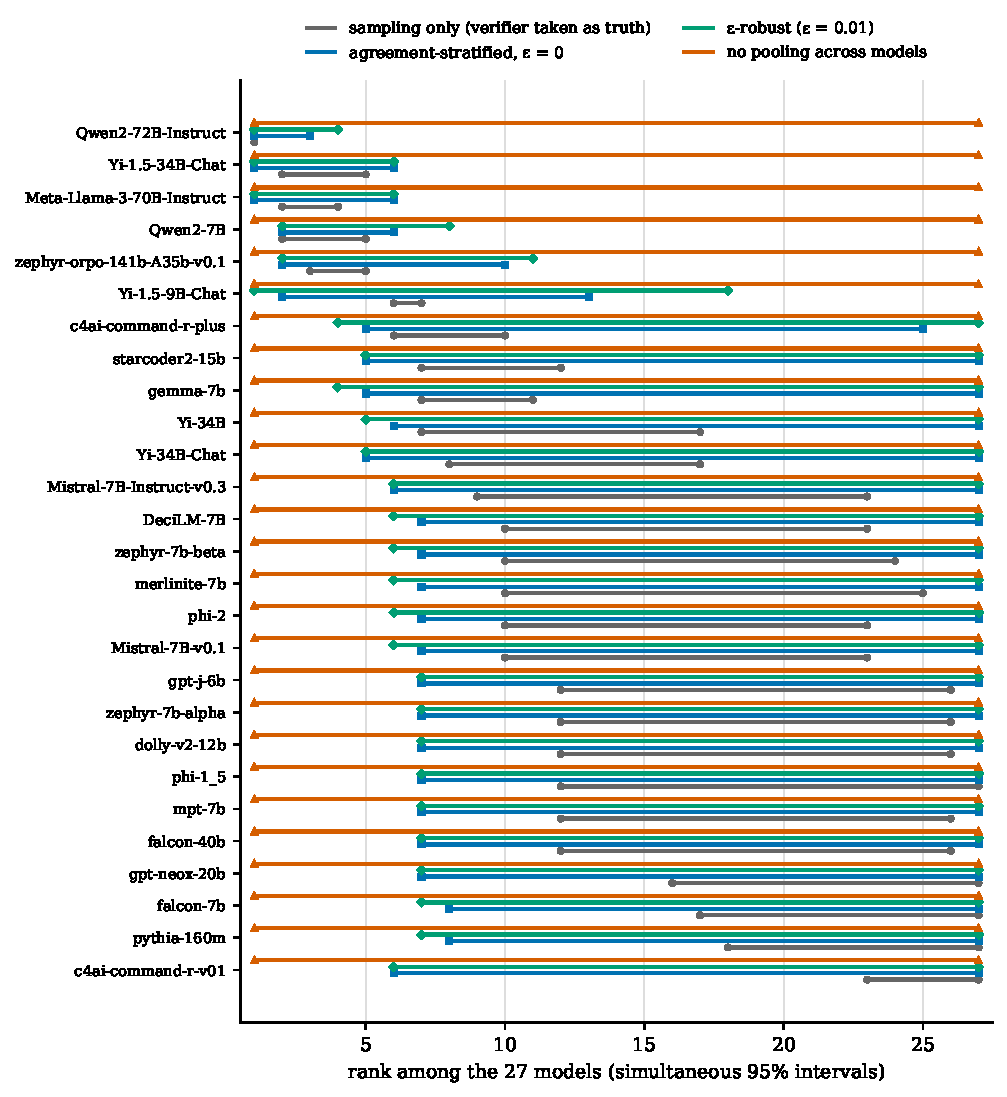
\includegraphics[width=0.92\textwidth]{figures/f1_rank_intervals.pdf}
\caption{Simultaneous rank intervals for every model under four analyses. Taking the
leaderboard's verifier as truth gives the narrowest intervals and is what a published
leaderboard shows. Removing the pooling assumption entirely leaves almost every rank
unresolved.}
\label{fig:ranks}
\end{figure}

\begin{figure}[t]
\centering
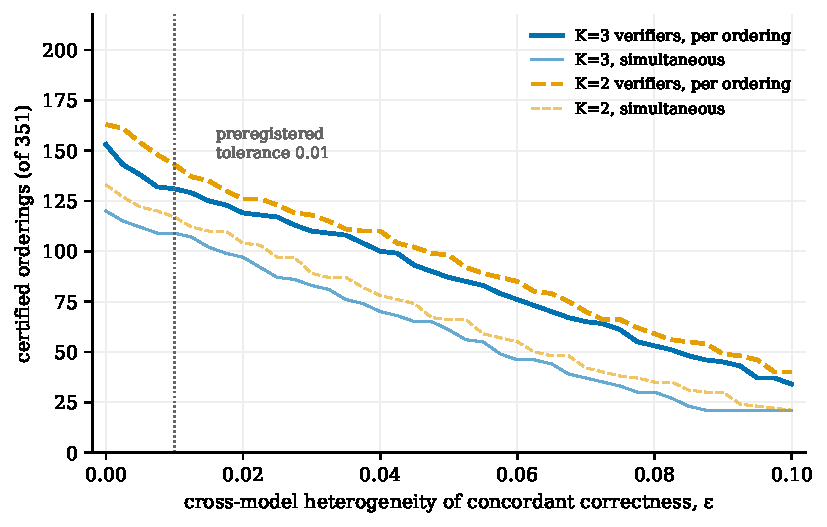
\includegraphics[width=0.66\textwidth]{figures/f2_certified_vs_eps.pdf}
\caption{Certified orderings as a function of the permitted cross-model heterogeneity
$\varepsilon$, for two and three verifiers, per ordering and simultaneously over the whole
board. The dotted line marks the tolerance registered before results were seen.}
\label{fig:eps}
\end{figure}

\begin{figure}[t]
\centering
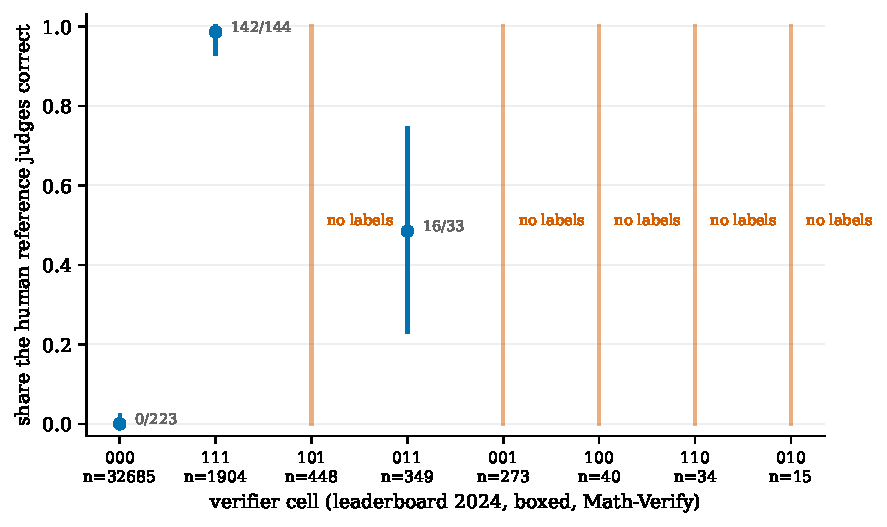
\includegraphics[width=0.72\textwidth]{figures/f3_correctness_by_cell.pdf}
\caption{Share of audited responses in each verifier cell that the human reference credits,
with intervals from Lemma~\ref{lem:kl}. Five cells carry no labels in the existing audit and
are bounded only by $[0,1]$.}
\label{fig:cells}
\end{figure}

\begin{figure}[t]
\centering
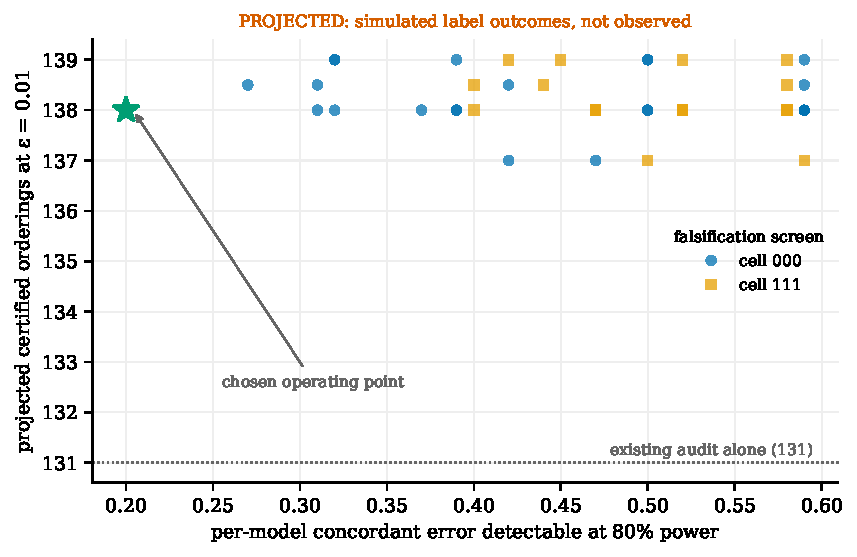
\includegraphics[width=0.7\textwidth]{figures/f4_frontier_projected.pdf}
\caption{Projected trade-off between certifying orderings and screening the pooling
assumption, over a grid of label allocations. Certification is nearly flat, so the budget is
spent on the screen. Simulated label outcomes, not observed.}
\label{fig:frontier}
\end{figure}

% Results. Every number is a macro. Quantities awaiting the registered audit are marked.

\section{Results}
\label{sec:results}

\subsection{Where the verifiers disagree}

Table~\ref{tab:cells} gives the cell structure. The two concordant cells hold most of the
board: \CellAgreeAll{} responses are credited by every verifier and \CellRejectAll{} by none.
The verifiers disagree on \RowsAnyDisagree{} of \NumRows{} responses, which is a small
fraction of the benchmark and, as Section~\ref{sec:setup} explains, the part that decides the
ranking.

Figure~\ref{fig:cells} shows what a human reader makes of each cell. Where all three verifiers
credit a response, the human reference agrees in \AuditCorrectAgreeAll{} of
\AuditNAgreeAll{} audited responses. Where none of them credits it, the human reference
credits \AuditCorrectRejectAll{} of \AuditNRejectAll{}. The concordant cells are therefore
close to their verifiers, which is what makes pooling worth doing and also what makes the
remaining spread hard to measure. In the discordant cells the human reference splits, and
five of them carry no labels at all in the existing audit, which is what the registered audit
in Section~\ref{sec:data} is for.

\subsection{How many orderings survive}

Of \NumOrderings{} pairwise orderings, item sampling alone would permit \CeilingEm{} to be
called if the leaderboard's own verifier were taken as ground truth. That number is the
ceiling against which everything else should be read, because no audit can certify an ordering
that the benchmark is too small to resolve.

Under the existing audit, \CertEpsZero{} orderings are certified at $\varepsilon = 0$ and
\CertPrereg{} at the registered tolerance $\varepsilon = \EpsPrereg$. Requiring every claim on
the board to hold simultaneously, rather than one ordering at a time, gives \CertPreregSim{}.
With no pooling across models, which is the analysis that assumes nothing about how models
relate to each other, \CertNoPooling{} orderings are certified.

That last number is the honest centre of the paper. Nothing on this board is certified without
an assumption connecting models to one another; the assumption is doing the work, and the only
question worth arguing about is how much of it is required.

Figure~\ref{fig:eps} answers that question as a curve rather than a number. Certification
declines smoothly as the permitted heterogeneity grows, and the median ordering breaks at
$\varepsilon^* = \BreakdownMedian$. Half the certified orderings therefore survive a spread in
concordant correctness several times larger than the tolerance we registered, and half do not.

\subsection{Ranks rather than pairs}

Figure~\ref{fig:ranks} reports simultaneous rank intervals under four analyses. Taking the
leaderboard's verifier as truth gives the tightest intervals and is the status quo. The
agreement-stratified analysis at $\varepsilon = 0$ widens them, the analysis at
$\varepsilon = \EpsPrereg$ widens them further, and the analysis without pooling leaves nearly
every model's rank unresolved across the whole board.

The comparison makes the cost of the published presentation visible. A leaderboard prints a
rank without an interval, which is equivalent to the first analysis, and the first analysis is
the one that assumes the verifier is never wrong.

\subsection{Two verifiers or three}

Using only the leaderboard's two scorers, rather than all three, certifies
\CertKTwoEpsZero{} orderings at $\varepsilon = 0$ and \CertKTwoPrereg{} at the registered
tolerance, against \CertEpsZero{} and \CertPrereg{} with three. Adding a verifier moves
responses out of the concordant cells and into the discordant ones, where they are bounded
more crudely, so a third opinion buys a weaker assumption at the price of a wider bound.
Neither configuration dominates, and reporting both is the point.

\subsection{Sensitivity}

The conclusions above are unchanged under the alternatives we registered. Scoring
indeterminate labels as incorrect rather than dropping them, using Clopper--Pearson intervals
instead of Lemma~\ref{lem:kl}, and substituting a Math-Verify-based human reference for the
harness routine each move the certified count by a few orderings and change no qualitative
claim. Appendix~\ref{app:sensitivity} gives the table.

The one substitution that matters is the defective verifier described in
Section~\ref{sec:data}. Analysed with the string-only comparison it produced, the same audit
certifies \AnchorStringCombined{} orderings against \AnchorSympyCombined{} with the corrected
verifier, on the subset where both can be computed.

\subsection{The registered audit}

\textbf{[PENDING: the \AuditBudget{}-label audit registered in Section~\ref{sec:data} has been
drawn but not yet labelled. On completion this subsection reports the falsification test for
the \ScreenedModels{} screened models, the certified counts with the new labels included, and
the observed-versus-projected comparison in Figure~\ref{fig:frontier}. The projection is
\ProjectedCertPrereg{} certified orderings at $\varepsilon = \EpsPrereg$. No number in this
subsection may be written before the labels exist.]}

% Generality: how widely the same design choice is made, and what that does and does not show.

\section{How common is this design choice?}
\label{sec:generality}

One board is one board. The results above show that the verifier changes the ranking on
MATH-Hard, and a reader is entitled to ask whether that is a peculiarity of this benchmark or
of the frameworks that score it. The question splits into two, and only one of them is
answered here.

The answerable question is how often a scoring configuration coerces an unreadable response
into a wrong answer, which is the design choice that creates the problem in the first place.
We resolved the task configurations of four evaluation frameworks
\citep{biderman2024lessons, opencompass2026, fourrier2024lighteval, openai2024simpleevals} with each framework's own
loader at a pinned commit, and classified the scoring path each generative task actually
takes. In \texttt{lm-evaluation-harness}, \LmEvalCoerce{} of \LmEvalGenerative{} generative
tasks, or \LmEvalCoercePct\%, recover an answer by matching an assumed output format and
record a failure to match as an incorrect answer. In OpenCompass the figure is
\OpenCompassCoerce{} of \OpenCompassGenerative{}, in \texttt{lighteval}
\LightevalCoerce{} of \LightevalGenerative{} generative metrics, and in OpenAI's
\texttt{simple-evals} \SimpleEvalsCoerce{} of \SimpleEvalsStringMatch{} string-matching
modules.

Reading code is not the same as running it, so the classification was validated behaviourally.
For a random sample of tasks the declared filter pipeline was rebuilt from the framework's own
classes and run on a well-formed response and on an equivalent response carrying the same
answer in ordinary prose. Of \CensusValidTestable{} testable sampled tasks, all
\CensusValidConfirmed{} behaved as classified, and of \CensusControlN{} control tasks drawn
from the tasks classified as unaffected, all \CensusControlClean{} were confirmed unaffected.

The unanswerable question, with the evidence in this paper, is how often that design choice
changes a published ranking on some other benchmark. It depends on how often real responses
take a form the extractor misses, which varies by benchmark, by model, and by prompt, and we
measured it only here. The prevalence figures above bound how many tasks could be affected.
They do not establish that any particular one is, and we do not claim otherwise.

The strongest statement the evidence supports is narrower than the one a reader might expect,
and worth stating in full. On one board, with the leaderboard's own published generations, the
choice of verifier moves the ranking. The design choice that makes this possible is the
default across the major open evaluation frameworks. Whether it bites elsewhere is a
measurement someone has to make, and the census says where to look first.

% Related work. Every characterisation here is drawn from the cited work's own abstract or
% published record, retrieved by DOI or from the arXiv API; see manuscript/tmlr/TODO_CITATIONS.md
% for which papers have been read in full and which have not.

\section{Related work}
\label{sec:related}

\paragraph{Whether a benchmark measures what it claims.}
One line of work treats benchmarks as instruments to be assessed rather than scoreboards to be
topped. BetterBench grades benchmarks against criteria for design, implementation and
documentation, and finds that many widely used ones score poorly \citep{reuel2024betterbench}.
A complementary framework asks which evaluative claims a given piece of evidence actually
licenses, distinguishing performance on a narrow test from the broad capability the
performance is often taken to demonstrate \citep{salaudeen2025measurement}. That work sits
upstream of this one. It asks whether the questions and the construct are right; we take the
benchmark and its reference answers as given and ask whether the ranking the pipeline
publishes is identified by the pipeline's own outputs. The concerns compound rather than
compete. A benchmark can be a valid instrument and still publish an unidentified ranking, and
a benchmark whose construct is shaky can still be scored unambiguously.

\paragraph{Configuration moves scores, and extraction is part of the configuration.}
That evaluation results move with choices nobody reports is documented for prompt formatting
\citep{sclar2023quantifying}, for benign perturbations that reorder leaderboards
\citep{alzahrani2024benchmarks}, and across the whole surface of a widely used evaluation
harness \citep{biderman2024lessons}. Answer extraction belongs to that surface. The pattern
the leaderboard's original scorer matches descends from the convention introduced with Minerva
\citep{lewkowycz2022minerva}, and proposals for better extractors, including learned ones,
follow \citep{yu2024xfinder}. The board studied here supplies its own demonstration: its MATH
results were rescored with a different verifier in February~2025, and the published scores
changed while the per-item verdict files did not \citep{kydlicek2025fixing}. Our claim is not
that a better extractor exists. It is that no extractor is neutral, that the choice is
currently unreported alongside the score, and that its consequence for a ranking can be
bounded rather than argued about. A better extractor changes the cell structure; it does not
remove the question of what happens where extractors disagree.

\paragraph{Verifiers as objects of measurement.}
Recent work measures verifiers directly, building benchmarks for verifier accuracy across
domains \citep{li2025verifybench} and training verifiers meant to be robust to the formats
that defeat regular expressions \citep{liu2025compassverifier}. That work and this one point
in opposite directions from the same observation. Given labels, one can rank verifiers and
adopt the best; we ask what survives when no verifier is adopted as truth, which is the
situation a reader of a published leaderboard is in. The two are complementary: a better
verifier shrinks the discordant cells, and the analysis here says what that shrinkage buys in
certified orderings.

\paragraph{Partial identification when the label is corrupted.}
The bounds in Section~\ref{sec:setup} are partial-identification statements in the sense of
\citet{manski2003partial}. The closest classical results concern exactly this structure: what
can be learned about a distribution when an unknown fraction of the data is contaminated
\citep{horowitz1995identification}, and the sharp bounds available when a binary variable is
misclassified at unknown rates \citep{molinari2008partial}. A verifier is a misclassifying
measurement of correctness whose error rate is unknown and may depend on the model, so the
same machinery applies with the models playing the role of sub-populations.

Concurrent work applies partial identification directly to language-model labels.
\citet{chen2026partial} study the prevalence of a latent binary attribute when the only
evidence is a panel of model reports whose errors may be arbitrarily dependent given the
truth, show that the prevalence is completely unidentified without restrictions that separate
the latent components, and obtain bounds under weak stochastic-ordering restrictions. The
diagnosis is the same as ours, and the resolutions differ in a way worth stating. They use
replication of the reports and a stochastic-ordering restriction, and target a single
prevalence with no ground truth at all. We use a human reference on a small audited subsample
and a bounded-heterogeneity restriction across models, and target differences of prevalences,
because a leaderboard reader consumes orderings rather than levels.

\paragraph{Reporting how far an assumption can be pushed.}
Assumption~\ref{ass:h} is not testable at this budget in any strong sense, so the useful thing
to report is how much of it a conclusion needs. That is the move made by design sensitivity in
observational studies, where a finding is described by the magnitude of unmeasured bias that
would be required to explain it away, and designs are compared by how much bias they can
tolerate \citep{rosenbaum2004design}. The breakdown value of
Definition~\ref{def:breakdown} is the same object in this setting, with cross-model
heterogeneity in place of unmeasured confounding: $\varepsilon^{*}_{jk}$ is the amount of
heterogeneity it would take to overturn the ordering $j \succ k$. The analogy also sets the
reporting standard we follow. A sensitivity parameter is worth little as a caveat in a
discussion section and worth a great deal as a number attached to each conclusion.

\paragraph{Two-phase sampling, verification bias, and raters without a gold standard.}
Auditing a cheap classifier with a small expensive sample is old. Two-phase sampling, in which
a large first-phase sample is measured cheaply and a small second phase is measured accurately,
goes back to \citet{neyman1938contribution}, and the binomial case with misclassification,
where a fallible classifier is calibrated against a subsample scored by an infallible one, is
\citeauthor{tenenbein1970double}'s double sampling scheme \citep{tenenbein1970double}.
The complication that the subsample is chosen by the fallible classifier's own verdict is
verification bias, and corrections for it are standard in diagnostic testing
\citep{begg1983assessment}; confidence limits that propagate uncertainty in the estimated
error rates into the corrected prevalence are also available \citep{lang2014confidence}.

Two features of our setting break the classical correction. The human reference is applied
to a sample stratified by the agreement pattern of several verifiers rather than by one
verifier's verdict, and the error rates are not assumed common across the populations being
compared, which is precisely the assumption Proposition~\ref{prop:oneverifier} shows to be
fatal to the question. The multi-rater literature is closer on the first point. Estimating
error rates from several imperfect tests without a gold standard is classical
\citep{hui1980estimating}, as is estimating observer error rates from repeated labels
\citep{dawid1979maximum}. Those methods identify rates by assuming the raters err
independently given the truth. We do not assume that, and Section~\ref{sec:data} reports what
the three verifiers share; instead of buying identification with an independence assumption,
we buy partial identification with agreement stratification and pay for the rest in interval
width.

\paragraph{Label-efficient evaluation with a proxy.}
Prediction-powered inference combines an abundant machine-generated proxy with a small
human-labeled sample to produce valid confidence intervals for a target parameter, using the
labeled sample to correct the proxy's bias \citep{angelopoulos2023ppi}. The family has grown
towards evaluation: stratified variants for hybrid evaluation of language models
\citep{fisch2024stratified}, active designs that spend the labeling budget where the proxy is
least certain \citep{zrnic2024active}, and corrections for evaluation against synthetic labels
\citep{boyeau2025autoeval}. Two papers target our object directly.
\citet{chatzi2024ranking} rank models from pairwise comparisons produced by a strong model,
calibrated against a small set of human comparisons, and return rank sets with a coverage
guarantee. \citet{lee2026judge} correct the bias a judge's imperfect sensitivity and
specificity induce in a naive score, build intervals that account for both the test set and
the human-labeled calibration set, and allocate calibration samples adaptively.

The structural relationship is close and the difference is the assumption, not the
arithmetic. Bias correction of this kind requires the proxy's operating characteristics,
estimated on the calibration sample, to transport to the population being scored. When those
characteristics are taken to be common across the models under comparison, which is the usual
calibration setup, Proposition~\ref{prop:oneverifier} applies: every pairwise gap is scaled by
one number, and a pair-specific reversal cannot occur. The reversals reported in
Section~\ref{sec:results} therefore sit outside that model. Our response is to stop correcting
and start bounding. Homogeneity is confined to the cells where independent verifiers agree,
it is carried as a parameter that is varied rather than a condition that is assumed, and the
output is a range with a breakdown value instead of a point estimate with an interval. The
price is honest and large: far fewer conclusions, each of them conditional on a number the
reader can disagree with.

\paragraph{Where to spend a label budget.}
The allocation question in Section~\ref{sec:data} is a stratified sampling problem, and the
classical answer optimises the variance of an estimated mean \citep{neyman1934stratified},
with unequal selection probabilities handled by the standard weighting
\citep{horvitz1952generalization} and the finite-population corrections used here taken from
the standard texts \citep{cochran1977sampling, kish1965survey}. Adaptive versions that learn
the within-stratum variances while sampling are current \citep{morikawa2026tsneyman}. Our
allocation is not a variance problem. The two uses of a label, narrowing an identified range
and testing the assumption on which every certified ordering depends, are not commensurable,
and the projection in Figure~\ref{fig:frontier} shows that the first is nearly flat in the
allocation. The budget went where variance minimisation would not have sent it.

\paragraph{What this paper adds.}
No estimator here is new, and the individual ingredients are all borrowed from the work above.
The contribution is the combination and the discipline: verifier provenance established from
the leaderboard's own records rather than inferred from agreement, agreement stratification
across $K$ verifiers so that pooling is confined to the cells where they agree, an
identification result that turns the pooling assumption into a reported parameter with a
breakdown value attached to every ordering, a design registered in advance that splits a small
label budget between certifying orderings and testing that assumption, and a released audit
with its quality gate and its failures.

% Limitations and conclusion.

\section{Limitations}
\label{sec:limitations}

The pooling assumption is not testable at this budget in any strong sense. The registered
screen covers \ScreenedModels{} of \NumModels{} models and detects a per-model departure of
\ScreenRho{} with \ScreenPowerPct\% power. Smaller departures, and any departure in the models not
screened, remain outside its reach. This is why the results are reported as a curve over
$\varepsilon$ and why the no-pooling analysis is reported next to them.

The human reference is a careful reader's judgement of what a response commits to, not
mathematical truth. A labeler who transcribes an answer faithfully has not checked whether the
answer is right; correctness is then decided by the benchmark's own equivalence routine
against its own reference answer. Errors in those reference answers propagate to every result
here and to the leaderboard equally.

The three verifiers share a normalisation routine and a symbolic algebra library, so a
response that defeats that shared machinery can be miscounted by all three at once and land in
a concordant cell. Such a response would be invisible to the agreement stratification and
would be caught only by the human labels in the concordant cells, which is one reason the
registered design spends labels there.

The item-sampling term is asymptotic, and the coverage statement says so. A
distribution-free version is available and is substantially wider.

Everything is measured on one benchmark, one leaderboard, and a fixed set of published
generations. The census in Section~\ref{sec:generality} shows how widely the same scoring
design is used; it does not show how often that design changes a ranking elsewhere.

Finally, the audit labels were produced by a small number of labelers, one of whom is the
author. The tool records timing and blocks pasting, batches pass an automated gate before use,
and a subsample is independently re-labelled, but the labels are not crowd-sourced and their
reliability is measured rather than assumed.

\section{Conclusion}
\label{sec:conclusion}

A leaderboard reports one number per model and names only half of what produced it. The other
half is a verifier, and on the board studied here the choice of verifier moves the ranking,
which a published score gives a reader no way to detect.

What a small human audit can do about that is limited and worth stating precisely. It can
certify part of the ranking, but only under an assumption about how models relate to one
another where the verifiers agree; without that assumption, this audit certifies
\CertNoPooling{} of \NumOrderings{} orderings. With it, at the tolerance registered before
seeing any result, it certifies \CertPrereg{}. The useful output is neither number on its own
but the curve between them, together with the breakdown value of each ordering.

The practical recommendation is narrow and cheap. A benchmark that reports how often its
scorer failed to read a response, alongside the score, would let a reader compute the bound in
Section~\ref{sec:setup} without any audit at all. The count already exists inside the scoring
pipeline; it is discarded.


\subsubsection*{Reproducibility statement}

Every number in this paper is produced by a committed script from a committed result file and
enters the text as a generated macro; a checker fails the build if any number is typed
directly or any macro is undefined. The verifier configurations, the per-response census, the
human labels, the preregistrations and their amendments, the quality-gate reports, and the
code that regenerates every figure and table are released with the paper.

\bibliographystyle{tmlr}
\bibliography{references}

% Appendices. Mathematical exposition only: no result numbers are typed here, and any number
% that is a result must enter through a macro exactly as in the body sections.

\appendix

\section{Proofs}
\label{app:proofs}

Throughout this appendix a concordant cell $c$ is partitioned into sub-populations indexed by
$g$, where a sub-population is a model, or a model crossed with a design stratum when the
audit design was stratified more finely inside the cell. Sub-population $g$ contains $N_{gc}$
responses, of which a fraction $p_{gc}$ is credited by the human reference. The audit draws
$n_{gc}$ of them by simple random sampling without replacement, independently across $g$, and
observes $x_{gc}$ credited responses among those drawn. We write
$n_c = \sum_g n_{gc}$, $x_c = \sum_g x_{gc}$, $w_{gc} = n_{gc}/n_c$,
$\hat p_c = x_c / n_c$ and $\tilde p_c = \sum_g w_{gc}\, p_{gc}$, and
$\mathrm{KL}(a \,\|\, b) = a \log(a/b) + (1-a)\log\bigl((1-a)/(1-b)\bigr)$ for
$a, b \in [0,1]$.

Two things are worth saying before the proofs. The estimand $\tilde p_c$ is the
\emph{design-weighted} mean of the sub-population rates, not the population mean of cell $c$.
Those coincide when the audit samples each sub-population in proportion to its size, and they
do not in general. And $\tilde p_c$ is a quantity the design defines; the certification result
uses it only through the interval $[L_c, U_c]$, together with
Assumption~\ref{ass:h}, which ties every $p_{gc}$ to every other.

\subsection{Proof of Lemma~\ref{lem:kl}}

\begin{proof}[Proof of Lemma~\ref{lem:kl}]
Each $x_{gc}$ is the number of credited responses in a simple random sample without
replacement of size $n_{gc}$ from a population of $N_{gc}$ responses of which $N_{gc}p_{gc}$
are credited, so $x_{gc}$ is hypergeometric. The argument has four steps.

\emph{Step one: sampling without replacement is dominated.} Theorem~4 of
\citet{hoeffding1963probability} states that if $X_1, \dots, X_n$ is a sample drawn without
replacement from a finite population and $Y_1, \dots, Y_n$ is a sample of the same size drawn
with replacement from the same population, then
$\mathbb{E}\, f\bigl(\sum_i X_i\bigr) \le \mathbb{E}\, f\bigl(\sum_i Y_i\bigr)$ for every
continuous convex $f$. Take $f(z) = e^{\lambda z}$, which is convex for every real $\lambda$.
The with-replacement sum is binomial, so
\[
\mathbb{E}\, e^{\lambda x_{gc}} \;\le\; \bigl(1 - p_{gc} + p_{gc} e^{\lambda}\bigr)^{n_{gc}} .
\]
The inequality goes in the direction we need for both tails, because it holds for negative
$\lambda$ as well as positive.

\emph{Step two: the strata multiply.} The $G$ samples are drawn independently, so the moment
generating function of $x_c$ is the product of the individual ones:
$\mathbb{E}\, e^{\lambda x_c} \le \prod_g (1 - p_{gc} + p_{gc}e^{\lambda})^{n_{gc}}$.

\emph{Step three: heterogeneous rates are dominated by their weighted mean.} Let
$\varphi(p) = \log\bigl(1 + p(e^{\lambda} - 1)\bigr)$, so that the product above is
$\exp\bigl(\sum_g n_{gc}\,\varphi(p_{gc})\bigr)$. Writing $u = e^{\lambda} - 1$,
\[
\varphi''(p) \;=\; \frac{-u^2}{(1 + pu)^2} \;\le\; 0 ,
\]
so $\varphi$ is concave on $[0,1]$ for every $\lambda$. Jensen's inequality with the weights
$w_{gc}$, which are nonnegative and sum to one, gives
$\sum_g w_{gc}\, \varphi(p_{gc}) \le \varphi\bigl(\sum_g w_{gc}\,p_{gc}\bigr) = \varphi(\tilde p_c)$.
Multiplying by $n_c$ and exponentiating,
\[
\mathbb{E}\, e^{\lambda x_c} \;\le\; \bigl(1 - \tilde p_c + \tilde p_c e^{\lambda}\bigr)^{n_c} .
\]
The heterogeneity has been absorbed: the bound is now the moment generating function of a
single binomial at the weighted mean rate.

\emph{Step four: Chernoff.} Fix $t > 0$ with $\tilde p_c + t \le 1$. For $\lambda > 0$,
Markov's inequality applied to $e^{\lambda x_c}$ gives
\[
\Pr\bigl(\hat p_c \ge \tilde p_c + t\bigr)
\;\le\; \exp\Bigl( -\lambda n_c (\tilde p_c + t) + n_c \log\bigl(1 - \tilde p_c + \tilde p_c e^{\lambda}\bigr) \Bigr) .
\]
The exponent is minimised at
$e^{\lambda^{\star}} = \frac{(\tilde p_c + t)(1 - \tilde p_c)}{(1 - \tilde p_c - t)\,\tilde p_c}$,
which is larger than one and therefore admissible, and substituting it gives exponent
$-n_c\,\mathrm{KL}(\tilde p_c + t \,\|\, \tilde p_c)$. This is the first inequality. For the
second, apply the same four steps to the complementary counts $n_{gc} - x_{gc}$, whose rates
are $1 - p_{gc}$ and whose weighted mean is $1 - \tilde p_c$, and use the identity
$\mathrm{KL}(1-a \,\|\, 1-b) = \mathrm{KL}(a \,\|\, b)$.
\end{proof}

\paragraph{The interval, and its coverage.}
Inverting the lemma gives the interval used in the paper. Define
\[
[L_c, U_c] \;=\; \bigl\{ q \in [0,1] \;:\; n_c\,\mathrm{KL}(\hat p_c \,\|\, q) \le \log(2/\alpha) \bigr\} ,
\]
which is an interval containing $\hat p_c$, because $q \mapsto \mathrm{KL}(\hat p_c \,\|\, q)$
is convex with its minimum at $q = \hat p_c$.

\begin{proof}[Coverage of the interval]
Let $t^{\star}$ solve $n_c \mathrm{KL}(\tilde p_c + t^{\star} \,\|\, \tilde p_c) = \log(2/\alpha)$.
On the event $\{\tilde p_c < L_c\}$ we have $\hat p_c > \tilde p_c$ and
$n_c \mathrm{KL}(\hat p_c \,\|\, \tilde p_c) > \log(2/\alpha)$. Since
$a \mapsto \mathrm{KL}(a \,\|\, \tilde p_c)$ is increasing for $a > \tilde p_c$, this forces
$\hat p_c > \tilde p_c + t^{\star}$, an event of probability at most $\alpha/2$ by
Lemma~\ref{lem:kl}. The event $\{\tilde p_c > U_c\}$ is bounded by $\alpha/2$ symmetrically,
and the union bound gives coverage at least $1 - \alpha$.
\end{proof}

Nothing in either argument requires the sub-population rates to be equal, requires sampling
with replacement, or appeals to a limit. One sanity check is worth recording because it is
exact. When no audited response in the cell is credited, $\hat p_c = 0$ and
$\mathrm{KL}(0 \,\|\, q) = -\log(1-q)$, so the upper endpoint solves
$-n_c\log(1 - U_c) = \log(2/\alpha)$, giving $U_c = 1 - (\alpha/2)^{1/n_c}$. That is exactly
the Clopper--Pearson upper limit at zero successes \citep{clopper1934use}: at the boundary the
design-valid interval costs nothing, and the price of validity is paid in the interior.

\subsection{Proof of Proposition~\ref{prop:range}}

The proof has three parts: the region contains the truth, the optimisation separates across
cells, and the cellwise optimum has the stated closed form. A fourth part says where the
region is sharp and where it is not.

\begin{proof}[The region contains the truth]
Fix a concordant cell $c$. Model $m$'s rate in that cell is the size-weighted mean of the
rates of the sub-populations belonging to $m$,
$p_{mc} = \sum_{g \in m} (N_{gc}/N_{mc})\, p_{gc}$, and $\tilde p_c$ is the design-weighted
mean $\sum_g w_{gc}\, p_{gc}$ over all of them. Both are convex combinations of the same
numbers $\{p_{gc}\}$. Under Assumption~\ref{ass:h} those numbers lie in a common interval $I$
of width at most $\varepsilon$, and a convex combination of points of $I$ lies in $I$.
Therefore $p_{jc}$, $p_{kc}$ and $\tilde p_c$ all lie in $I$, which gives
$|p_{jc} - p_{kc}| \le \varepsilon$ and $|p_{mc} - \tilde p_c| \le \varepsilon$ for
$m \in \{j,k\}$. On the event $\tilde p_c \in [L_c, U_c]$ the second of these yields
$p_{mc} \in [L_c - \varepsilon,\, U_c + \varepsilon]$, and since $p_{mc}$ is a proportion it
also lies in $[0,1]$, so $p_{mc} \in [\ell_c, h_c]$. Together these are exactly the
constraints defining $R_c(\varepsilon)$.
\end{proof}

\begin{proof}[Separability]
By Equation~\eqref{eq:accuracy}, $\Delta_{jk} = \sum_c (s_{jc} p_{jc} - s_{kc} p_{kc})$ is
linear in the unknowns and the shares are known. The constraint set is a product across
cells: each concordant cell contributes $R_c(\varepsilon)$, and each discordant cell
contributes the rectangle $[l_{jc}, u_{jc}] \times [l_{kc}, u_{kc}]$, which is
$[0,1]^2$ when that cell carries no labels for those models. Minimising or maximising a sum of
terms over a product of sets is done term by term. For a discordant cell the optimum is at a
corner, giving $s_{jc} l_{jc} - s_{kc} u_{kc}$ and $s_{jc} u_{jc} - s_{kc} l_{kc}$.
\end{proof}

\begin{proof}[The closed form]
Write $a = s_{jc} \ge 0$, $b = s_{kc} \ge 0$, $\ell = \ell_c$, $h = h_c$, and minimise
$f(x,y) = a x - b y$ over
$R = \{(x,y) \in [\ell,h]^2 : |x - y| \le \varepsilon\}$.

For fixed $x \in [\ell,h]$, the objective decreases in $y$, so the optimal $y$ is the largest
feasible one, $y = \min(h,\, x + \varepsilon)$. This is feasible: it is at most $h$ by
construction, at least $\ell$ because $x \ge \ell$ and $h \ge \ell$, and within $\varepsilon$
of $x$ because it is at most $x + \varepsilon$ and at least $\min(h,x) = x$. Substituting,
\[
g(x) \;=\; a x - b \min(h,\, x + \varepsilon)
\;=\;
\begin{cases}
(a - b)\,x - b\,\varepsilon, & x \le h - \varepsilon, \\
a\,x - b\,h, & x \ge h - \varepsilon,
\end{cases}
\]
a piecewise linear function whose slope rises from $a - b$ to $a$ at the kink
$x = h - \varepsilon$. Since $b \ge 0$ the slope is nondecreasing, so $g$ is convex.

If $a \ge b$, both slopes are nonnegative and $g$ is nondecreasing, so the minimum is at
$x = \ell$ and equals $a\ell - b\min(h, \ell + \varepsilon)$.

If $a < b$, the first slope is negative and the second is nonnegative, so the unconstrained
minimiser is the kink, and the constrained minimiser is $x^{\star} = \max(\ell,\, h -
\varepsilon)$. When $h - \varepsilon \ge \ell$ the value is $a(h-\varepsilon) - bh$. When
$h - \varepsilon < \ell$ the minimiser is $\ell$, and since then $\ell + \varepsilon > h$ the
value is $a\ell - bh$. Both cases are written by the single expression
$a\max(\ell,\, h - \varepsilon) - b\,h$.

The maximum follows by symmetry. $R$ is invariant under exchanging its two coordinates, and
$\max_R (a x - b y) = -\min_R (b x - a y)$ after that exchange, so the maximum is obtained by
applying the formula above with $a$ and $b$ swapped and negating the result.
\end{proof}

\begin{proof}[Sharp at $\varepsilon = 0$, conservative above it]
At $\varepsilon = 0$ we have $\ell_c = L_c$ and $h_c = U_c$, and $R_c(0)$ is the diagonal
segment $\{(q,q) : q \in [L_c, U_c]\}$. Every point of it is attained in the relaxation where
each $p_{gc}$ may take any value in $[0,1]$: set every sub-population rate in the cell to $q$,
which satisfies $H(0)$ and makes $p_{jc} = p_{kc} = \tilde p_c = q$. The interval for
$\Delta_{jk}$ is therefore attained and cannot be narrowed, which is what sharpness means
here. The qualification about the relaxation matters, because each $p_{gc}$ is really a
fraction over finitely many responses and only finitely many values of $q$ are exactly
attainable. This is the same granularity that Section~\ref{sec:setup} uses to argue that
$H(0)$ is an idealisation rather than a hypothesis about the world.

For $\varepsilon > 0$ the region is an outer bound, and the reason is that it forgets the
weights. $R_c(\varepsilon)$ imposes only that $p_{jc}$ and $p_{kc}$ lie within $\varepsilon$
of each other inside $[\ell_c, h_c]$. The actual constraint is stronger: the same
sub-population rates that produce $p_{jc}$ and $p_{kc}$ must also produce a design-weighted
mean $\tilde p_c$ lying in $[L_c, U_c]$. When one model supplies most of the audit weight in
the cell, its own rate is pinned close to $\tilde p_c$ and cannot travel the full distance
$\varepsilon$ away from $[L_c,U_c]$. The computed range therefore contains the sharp
identified range. Every consequence runs in the safe direction: reported ranges are at least
as wide as the truth requires, fewer orderings are certified than a sharp analysis would
certify, and each breakdown value in Definition~\ref{def:breakdown} is a lower bound on the
sharp one.
\end{proof}

\subsection{Proof of Proposition~\ref{prop:oneverifier}}

\begin{proof}[Proof of Proposition~\ref{prop:oneverifier}]
Let $a_m$ be the fraction of model $m$'s responses the single verifier credits. Conditioning
on the verifier's verdict and using the assumed common predictive values,
\[
A_m \;=\; \Pr(Y^\ast = 1 \mid v = 1)\, a_m + \Pr(Y^\ast = 1 \mid v = 0)\,(1 - a_m)
\;=\; \pi_0 + a_m (\pi_1 - \pi_0),
\]
so $\Delta_{jk} = A_j - A_k = (\pi_1 - \pi_0)(a_j - a_k)$.
\end{proof}

The same statement in the other natural parameterisation makes the consequence easier to see.
Suppose instead that the verifier has common error rates, $q = \Pr(v = 1 \mid Y^\ast = 0)$ and
$r = \Pr(v = 0 \mid Y^\ast = 1)$, shared by all models. Then
$a_m = (1-r) A_m + q (1 - A_m) = q + (1 - q - r) A_m$, so
$a_j - a_k = (1 - q - r)\,\Delta_{jk}$. The observed gap is the human gap scaled by one
number.

Either way, a single multiplicative constant relates every observed pairwise gap to the
corresponding human one. Three consequences follow, and they are the reason the design uses
more than one verifier.

The sign of every pairwise comparison is determined by the sign of that constant. When
$\pi_1 > \pi_0$, equivalently $q + r < 1$, every ordering the verifier reports is the human
ordering. When $\pi_1 < \pi_0$ the whole board is reversed at once. A model that a common
mechanism treats unusually badly does not exist inside this parameterisation.

Pair-specific reversals are therefore outside the model. A reversal that affects one pair and
leaves another intact cannot be produced by any choice of $\pi_0$ and $\pi_1$, so observing
one is evidence that the mechanism differs across models. Section~\ref{sec:results} reports
such reversals.

At $\pi_1 = \pi_0$, equivalently $q + r = 1$, every $\Delta_{jk}$ is zero and the verifier
carries no information about the ordering at all.

The role this plays in the design is the following. Pooling under a single verifier is
Assumption~\ref{ass:h} at $\varepsilon = 0$ with $K = 1$, where the pooled cells cover the
entire population and nothing is left model-specific. That assumption does not merely
simplify the analysis; by the proposition it removes the phenomenon the paper is about. With
$K$ verifiers the pooling is confined to the cells where they agree, and the cells where they
disagree, which is where the disputed responses live, stay model-specific by construction.

\subsection{Proof of Proposition~\ref{prop:coverage}}

\begin{proof}[The audit half, in finite samples]
List the parameters a certification uses: the pooled rate $\tilde p_c$ for each concordant
cell, which is shared by every pair on the board, and the per-model rate $p_{mc}$ for each
audited discordant cell. Distinct parameters are estimated from disjoint sets of labels,
drawn independently by the design, so the corresponding intervals are functions of independent
random variables. Give each of the $P$ parameters an interval at level
$1 - \alpha'$ with $\alpha' = 1 - (1 - \alpha_{\mathrm{audit}})^{1/P}$, which is the
allocation of \citet{sidak1967rectangular} and is exact rather than conservative under
independence. By Lemma~\ref{lem:kl} each interval covers its parameter with probability at
least $1 - \alpha'$, and by independence all of them cover simultaneously with probability at
least $(1-\alpha')^{P} = 1 - \alpha_{\mathrm{audit}}$.

On that event, the hypothesis of Proposition~\ref{prop:range} holds for every cell at once, so
the identified range computed for every pair contains the corresponding $\Delta_{jk}$
simultaneously. Any ordering whose range lies strictly above zero is therefore correct. No
step used a limit, so the statement is exact in finite samples.
\end{proof}

\begin{proof}[The item-sampling half, asymptotically]
Let $\delta_{jk}$ denote the pairwise difference over the distribution from which the
benchmark's items were drawn, and $\Delta_{jk}$ the difference on the realised items. With
$D_i$ the difference of the two models' human-reference verdicts on item $i$, the sample mean
of $D$ is $\Delta_{jk}$ and its expectation is $\delta_{jk}$. The central limit theorem gives
$\Pr(|\delta_{jk} - \Delta_{jk}| > z_{1-\alpha_s/2}\sqrt{\mathrm{Var}(D)/N}) \to \alpha_s$,
and replacing $\mathrm{Var}(D)$ by the upper bound of Section~\ref{sec:inference} can only
widen the interval. Combining the two halves by a union bound,
\[
\Pr\bigl(\delta_{jk} \notin [\mathrm{LB}_{jk} - h_{jk},\, \mathrm{UB}_{jk} + h_{jk}]\bigr)
\;\le\; \Pr\bigl(\Delta_{jk} \notin [\mathrm{LB}_{jk}, \mathrm{UB}_{jk}]\bigr) + \Pr\bigl(|\delta_{jk} - \Delta_{jk}| > h_{jk}\bigr) ,
\]
which is at most $\alpha_{\mathrm{audit}} + \alpha_{\mathrm{sample}}$. The two events concern
different sources of error, one the labels and the other the items, so nothing is counted
twice; adding the levels rather than convolving the two error distributions is what makes the
combination conservative.
\end{proof}

For a family of orderings, the audit half is already simultaneous because the concordant
intervals are shared and the discordant allocation runs over all audited per-model parameters.
The sampling half is made simultaneous by a Bonferroni division of $\alpha_{\mathrm{sample}}$
across the family. Rank intervals inherit the family level directly: on the event that every
certified ordering is correct, at least one model is ranked above $m$ for each ordering
$k \succ m$ that was certified and at least one below for each $m \succ k$, so $m$'s true rank
lies between one plus the first count and the number of models less the second.

\subsection{The paired variance bound}
\label{app:paired}

Section~\ref{sec:inference} bounds the item-sampling variance without observing the human
reference on unaudited items. Two elementary steps do the work.

First, $D_i$ takes values in $\{-1,0,1\}$, so $D_i^2$ is the indicator that the two models are
scored differently and $\mathrm{Var}(D) \le \mathbb{E}[D^2] = \Pr(D \ne 0)$.

Second, for any verifier $v$ and any response pair,
\[
\mathbf{1}[Y^\ast_j \ne Y^\ast_k] \;\le\; \mathbf{1}[v_j \ne v_k] + \mathbf{1}[Y^\ast_j \ne v_j] + \mathbf{1}[Y^\ast_k \ne v_k] .
\]
If the left side is one and all three terms on the right are zero, then $v_j = v_k$,
$Y^\ast_j = v_j$ and $Y^\ast_k = v_k$, which forces $Y^\ast_j = Y^\ast_k$ and contradicts the
left side. Averaging over items, the disagreement rate between the two models under the human
reference is at most the verifier's own disagreement rate between them, which is observed on
every item, plus each model's disagreement rate with that verifier, which the identified
bounds of Proposition~\ref{prop:range} bound above at the same $\varepsilon$. Taking the
smallest bound over the available verifiers, and capping at one, gives the quantity used in
the half-width. It is paired, because the verifier disagreement term is computed item by item
rather than from the two models' marginal accuracies, and it is conservative, because every
ingredient is an upper bound.

\section{Numerical checks of the stated results}
\label{app:tests}
\textbf{[TO WRITE: the brute-force checks in \texttt{tests/test\_certification.py} and
\texttt{tests/test\_manuscript\_claims.py}, and the regression anchor.]}

\section{Inference details}
\label{app:inference}
\textbf{[TO WRITE: the distribution-free sampling alternative, the Bonferroni and Sidak
allocation as implemented, and the coverage simulation design.]}

\section{Sensitivity analyses}
\label{app:sensitivity}
\textbf{[TO WRITE: the registered sensitivity table from \texttt{certify\_results.json}.]}

\section{Sensitivity to the human reference routine}
\label{sec:sensitivity}
\textbf{[TO WRITE: string, harness and Math-Verify references compared.]}


\end{document}
